\chapter*{Proposition 4}
\label{prop:4}


\begin{figure*}[ht]
    \begin{center}
    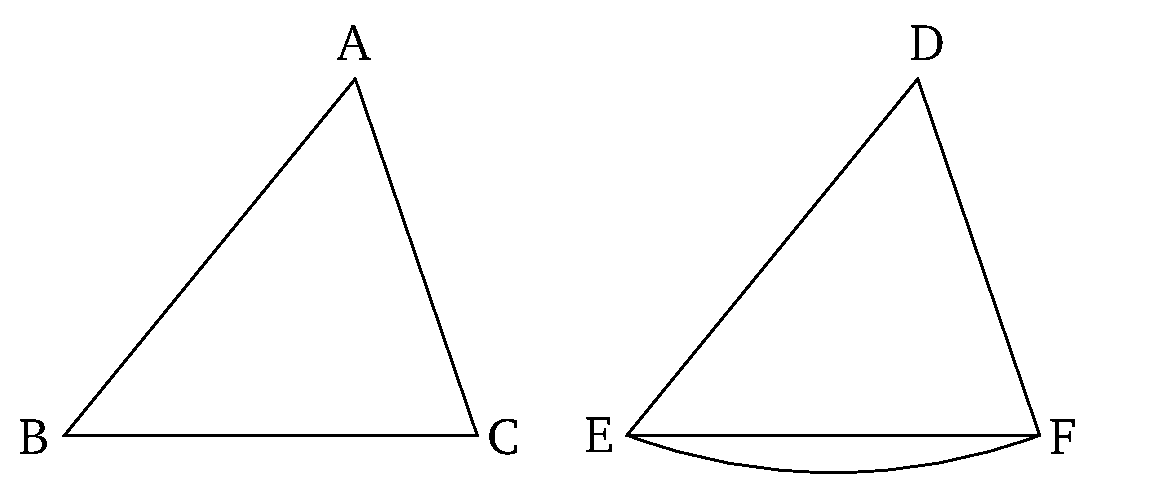
\includegraphics[width=0.5\linewidth]{figures/fig04e.eps}
    \label{fig:prop_4}
    \end{center}
\end{figure*}

If two triangles have two sides equal to two sides, respectively, and have the
angle(s) enclosed by the equal straight-lines equal, then
they will also have the base equal to the base, and the triangle will be equal
to the triangle, and the remaining angles subtended by the equal sides will be equal to the corresponding remaining angles.

Let $ABC$ and $DEF$ be  two triangles having the two sides $AB$ and $AC$ equal to the two sides $DE$ and $DF$, respectively. (That is) $AB$ to $DE$, and $AC$ to $DF$. And (let) the angle $BAC$ (be) equal to the angle $EDF$. I say that the base $BC$ is also equal to the base
$EF$, and triangle $ABC$ will be equal to triangle $DEF$, and the remaining angles
subtended by the equal sides will be equal to the corresponding remaining angles. (That is) $ABC$ to $DEF$, and $ACB$ to
$DFE$.

For if triangle $ABC$ is applied to triangle $DEF$, the point $A$ being placed
on the point $D$, and the straight-line $AB$ on $DE$, then the point $B$ will also coincide with $E$, on account of $AB$ being equal to $DE$. So (because of) $AB$ coinciding with $DE$, the straight-line $AC$ will also coincide with $DF$, on account of the angle $BAC$ being equal to $EDF$. So the point $C$ will also coincide with the
point $F$,  again on account of $AC$ being equal to $DF$.  But,  point $B$  certainly also coincided with point $E$, so that the base $BC$ will coincide with the base $EF$.
For if $B$ coincides with $E$, and $C$ with $F$, and the base $BC$ does not coincide with $EF$, then two straight-lines will encompass an area. The very thing is impossible [Post.~\ref{post:1}]. Thus, the base $BC$ will coincide with $EF$, and will be equal to it [C.N.~\ref{cn:4}]. So  the whole triangle $ABC$ will coincide with the whole triangle $DEF$, and will be equal to it [C.N.~\ref{cn:4}]. And the remaining angles will coincide with the remaining angles, and  will be equal to them [C.N.~\ref{cn:4}]. (That is) $ABC$ to $DEF$, and $ACB$
to $DFE$ [C.N.~\ref{cn:4}].

Thus, if two triangles have two  sides equal to two sides, respectively, and have the
angle(s) enclosed by the equal straight-line equal, then
they will also have the base equal to the base, and the triangle will be equal
to the triangle,  and
the remaining angles subtended by the equal sides will be equal to the
corresponding remaining angles. (Which is) the very thing it was required to show.


\section*{Commentary}

\begin{proposition}\label{proposition_4}\lean{Elements.Book1.proposition_4}\leanok
    $\triangle~ABC$ and $\triangle~DEF$ are two triangles with $|AB| = |DE|$, $|AC| = |DF|$, and $\angle~BAC = \angle~EDF$. Then, $\triangle~ABC$ and $\triangle~DEF$ must be congruent. That is, $|BC| = |EF|$, $\angle~ABC = \angle~DEF$, and $\angle~ACB = \angle~DFE$.
\end{proposition}
\begin{proof}
    \leanok
    See the original proof by Euclid.
\end{proof}
